\label{sec:results}

This section summarises what the experiment sequence revealed about reward shaping and action-space design.
Eval return and shutter behaviour are reported against the deterministic baseline anchor ($-38.6$); numbers above that anchor indicate a configuration learned useful scheduling on the fixed evaluation seed, not that the training problem is solved in general.

\subsection{Aggregate performance comparison}
\label{sec:results-aggregate}

Table~\ref{tab:results-summary} distils the closed experiments into a single snapshot of the design search.
The reference columns are the \textbf{deterministic baseline anchor} ($-38.6$) and the \textbf{best SAC configuration} (Exp~9, $+106.4$ on seed~7).

\begin{table}[htbp]
  \centering
  \caption{Aggregate results by experiment phase.
    Eval return is mean over 2 evaluation episodes on seed~7.
    $\Delta_\text{base}$ = eval return $-$ ($-38.6$) baseline anchor.
    Shutter cmds/ep: train mean where available.}
  \label{tab:results-summary}
  \begin{tabular}{lllrrr}
    \toprule
    Exp & Alg & Key change & Eval return & $\Delta_\text{base}$ & Shutter cmds/ep (train) \\
    \midrule
    Baseline anchor & --- & Fixed schedule     & $-38.6$ & --- & 10 (fixed) \\
    \midrule
    \multicolumn{6}{l}{\textit{Phase 1: Diagnosis}} \\
    1   & MPO & Threshold 0.5/0.9          & $-101.6$ & $-63.0$ & 516 \\
    2   & SAC & Compressed encoder         & $-78.9$  & $-40.3$ & 236 \\
    3   & SAC & Sparse reward              & $-22.2$  & $+16.4$ & --- \\
    3   & MPO & Dense reward               & $-51.6$  & $-13.0$ & --- \\
    5   & MPO & Width ablation (all)        & $-51.6$  & $-13.0$ & --- \\
    \midrule
    \multicolumn{6}{l}{\textit{Phase 2: Action space \& reward shaping}} \\
    4   & SAC & Torque mode (Ref0)         & $-11.1$  & $+27.5$ & --- \\
    4   & SAC & Vector mode (Ref1)         & $-24.1$  & $+14.5$ & 7071 \\
    7   & SAC & Vector + budget penalty    & $+10.6$  & $+49.2$ & 478 \\
    9   & SAC & Vector + budget, waste off & $+106.4$ & $+145.0$& --- \\
    \midrule
    \multicolumn{6}{l}{\textit{Phase 3: MPO stabilisation \& ablations}} \\
    8   & MPO & Decoupled-KL fix, torque   & $-81.1$  & $-42.5$ & --- \\
    10  & MPO & Safe-mode penalty ($k$=2.0)& $-510.4$ & $-471.8$& 2--7 \\
    11  & MPO & Fixed dual, vector         & $+45.5$  & $+84.1$ & 8--10 \\
    12  & MPO & Vector + effort ($k$=0.1)  & $+25.3$  & $+63.9$ & --- \\
    \midrule
    \multicolumn{6}{l}{\textit{Phase 4: Scale \& cadence}} \\
    13  & MPO & Cadence 1:1:50             & $-15.4$  & $+23.2$ & --- \\
    14  & MPO & Multi-env (crashed)        & n/a      & ---     & --- \\
    \bottomrule
  \end{tabular}
\end{table}

\subsection{Learning progression}
\label{sec:results-learning}

The episode-level learning curves show how the design space was narrowed:

\begin{itemize}
  \item \textbf{Exps~1--5:} Naive configurations (threshold tuning, encoder variants, algorithm and width ablations) produce flat or degrading returns.
    No run in this phase crosses positive territory, confirming that the training problem is not solved by default.
  \item \textbf{Exp~3:} SAC with sparse reward is the first configuration to show a rising training trajectory, establishing that the environment is learnable once the reward and algorithm pairing is correct.
  \item \textbf{Exp~7:} Adding a budget-exhausted shutter penalty to vector-mode SAC yields the first positive eval return ($+10.6$) and cuts train shutter commands from $\sim$7000 (Exp~4) to 478.
  \item \textbf{Exp~9:} Removing the within-budget waste penalty further improves eval return ($+106.4$).
    On eval episodes, two thirds of capture attempts are scientifically valid (non-cloud, within budget, previously uncaptured target).
  \item \textbf{Exp~11:} MPO in vector mode reaches $+45.5$, the first positive MPO eval return, after the decoupled-KL dual fix (Exp~8) removed the algorithm-level collapse.
\end{itemize}

\begin{figure}[htbp]
  \centering
  \begin{subfigure}[t]{0.48\linewidth}
    \centering
    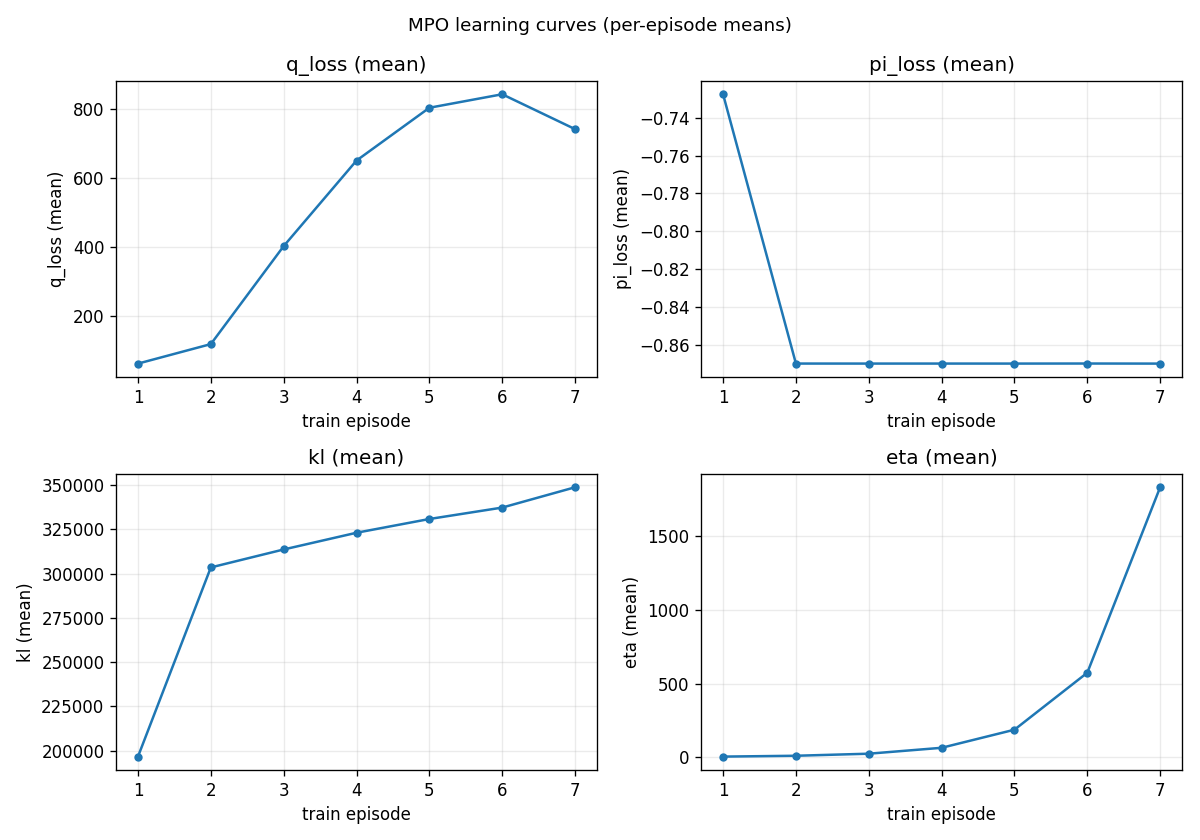
\includegraphics[width=\linewidth]{figures/fig_learning_curve_exp1.png}
    \caption{Exp~1 (not learning)}
  \end{subfigure}\hfill
  \begin{subfigure}[t]{0.48\linewidth}
    \centering
    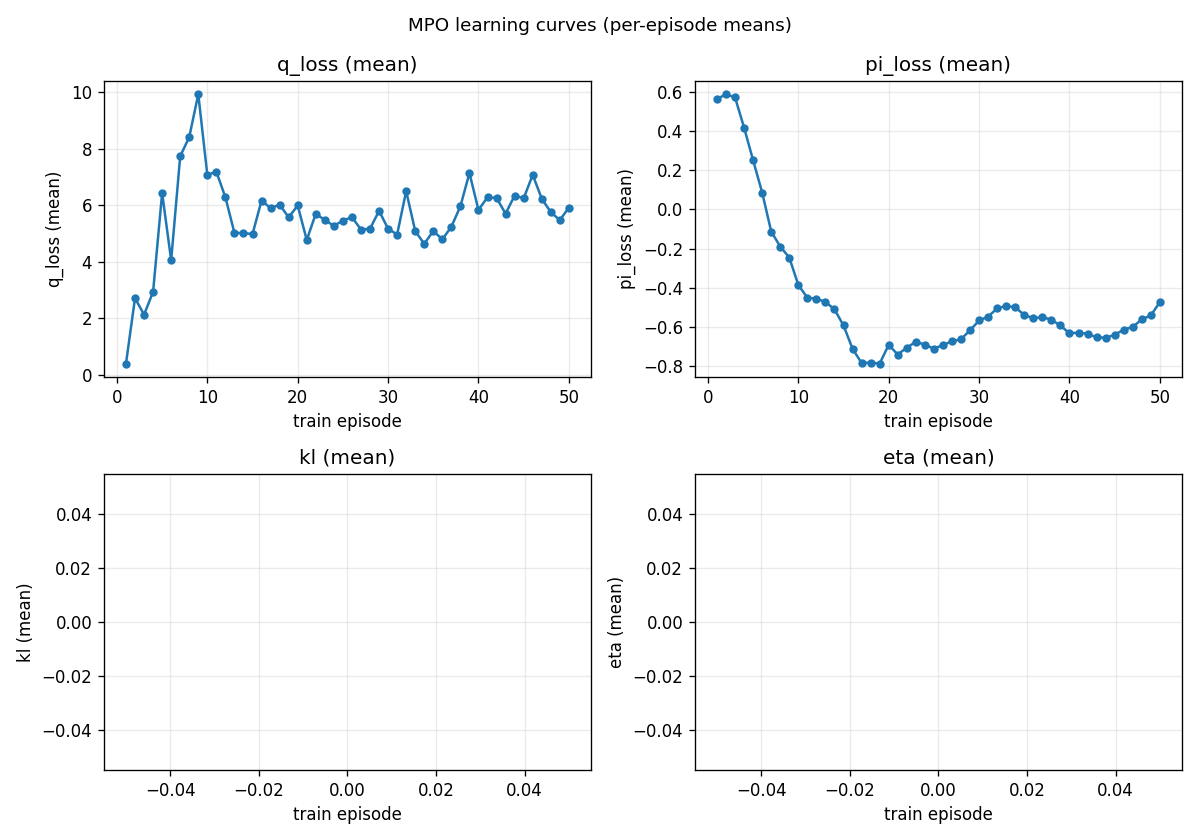
\includegraphics[width=\linewidth]{figures/fig_learning_curve_exp9.png}
    \caption{Exp~9 (learning)}
  \end{subfigure}
  \caption{Learning behaviour contrast: flat/collapsed training under Exp~1 shutter-threshold MPO versus rising returns under Exp~9 SAC shutter-split (best supported SAC configuration).}
  \label{fig:learning-vs-not}
\end{figure}

\begin{figure}[htbp]
  \centering
  \begin{subfigure}[t]{0.48\linewidth}
    \centering
    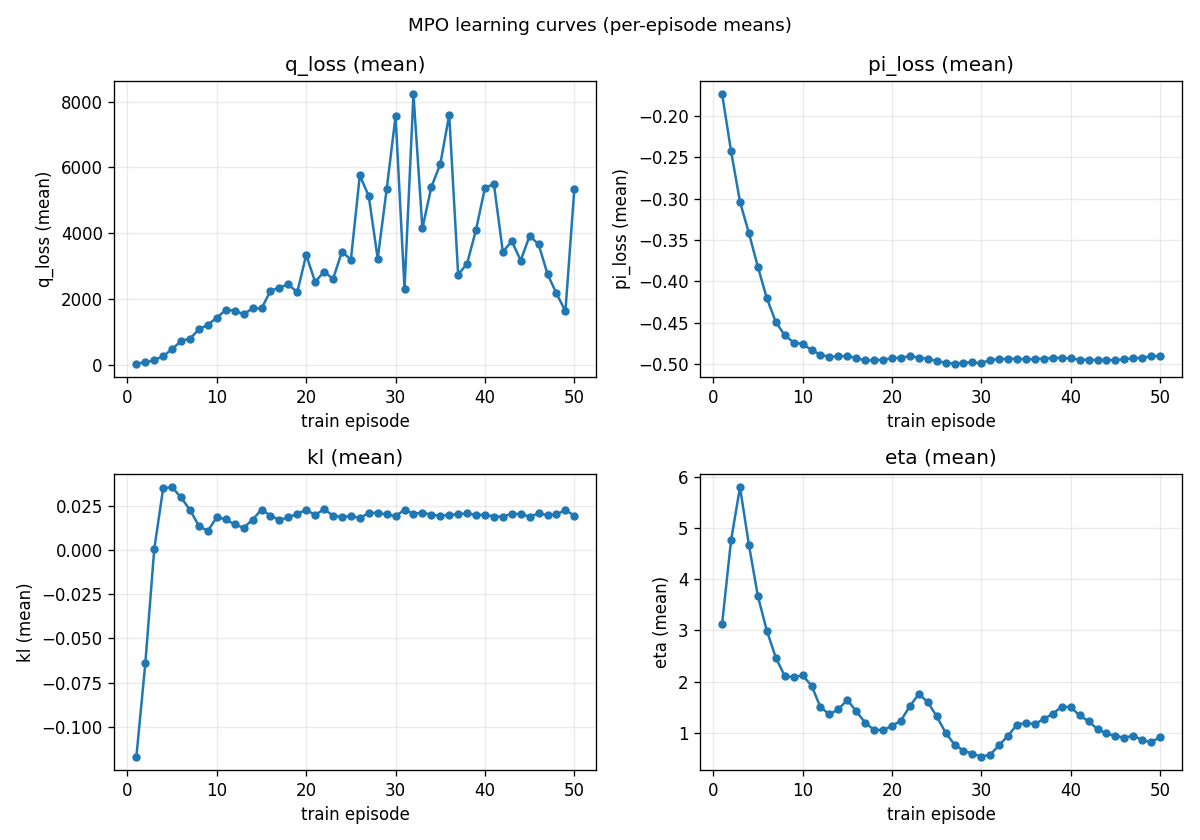
\includegraphics[width=\linewidth]{figures/fig_learning_curve_exp10.png}
    \caption{Exp~10 (not learning)}
  \end{subfigure}\hfill
  \begin{subfigure}[t]{0.48\linewidth}
    \centering
    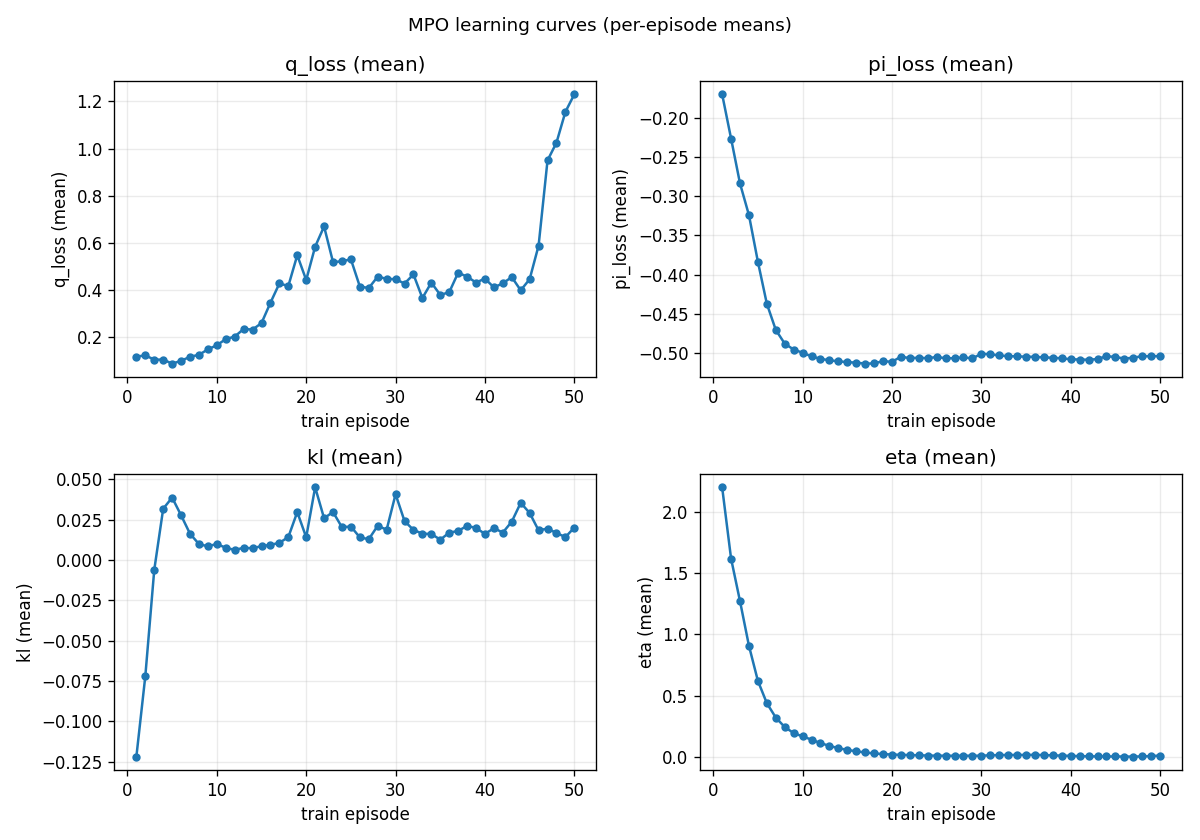
\includegraphics[width=\linewidth]{figures/fig_learning_curve_exp11.png}
    \caption{Exp~11 (learning)}
  \end{subfigure}
  \caption{MPO branch after the Exp~8 dual fix: Exp~10 safe-mode penalty collapses eval return, while Exp~11 vector-mode MPO shows sustained learning.}
  \label{fig:learning-mpo-contrast}
\end{figure}

\subsection{Shutter spam and budget efficiency}
\label{sec:results-shutter}

Shutter command count per episode tracks whether a policy has learned selective scheduling rather than firing continuously.
A well-trained policy would issue at most ten commands per episode (one per target within budget), timed to clear-sky windows.
The deterministic baseline issues exactly ten commands but ignores cloud content, so an estimated 30--40\% of its captures are wasted on cloud-blocked or empty targets.

Table~\ref{tab:shutter-progression} tracks the spam reduction path.

\begin{table}[htbp]
  \centering
  \caption{Shutter spam reduction across the SAC vector experiment chain.
    All figures are training means unless noted.}
  \label{tab:shutter-progression}
  \begin{tabular}{lrrl}
    \toprule
    Experiment & Cmds/ep (train) & Meaningful frac (train) & Notes \\
    \midrule
    Overnight H1a (pre-Exp~1) & 968 & 0 & MPO, threshold 0.5 \\
    Exp~1 mpo\_t05/t09         & 516 & 0 & Threshold ineffective \\
    Exp~4 Ref1 (SAC vector)    & 7071 & 0.015 & Budget ignorance \\
    Exp~7 (budget penalty)     & 478  & 0.220 & $-93\%$ cmds vs Ref1 \\
    Exp~9 (waste off)          & --- & 0.286 / 0.667 (eval) & Best scheduling \\
    Exp~11 (MPO vector)        & 8--10 & --- & Budget-aware MPO \\
    Baseline anchor (reference)  & 10  & $\sim$0.60--0.70 & Deterministic, cloud-blind \\
    \bottomrule
  \end{tabular}
\end{table}

The budget-exhausted penalty (Exp~7) was the single most impactful reward change in the series:
a 93\% reduction in shutter commands with a simultaneous increase in eval return.
Removing the waste penalty (Exp~9) added a further behavioural improvement on top of that configuration.
Together, these results show that reward structure, not algorithm choice alone, determines whether selective shuttering emerges.

\begin{figure}[htbp]
  \centering
  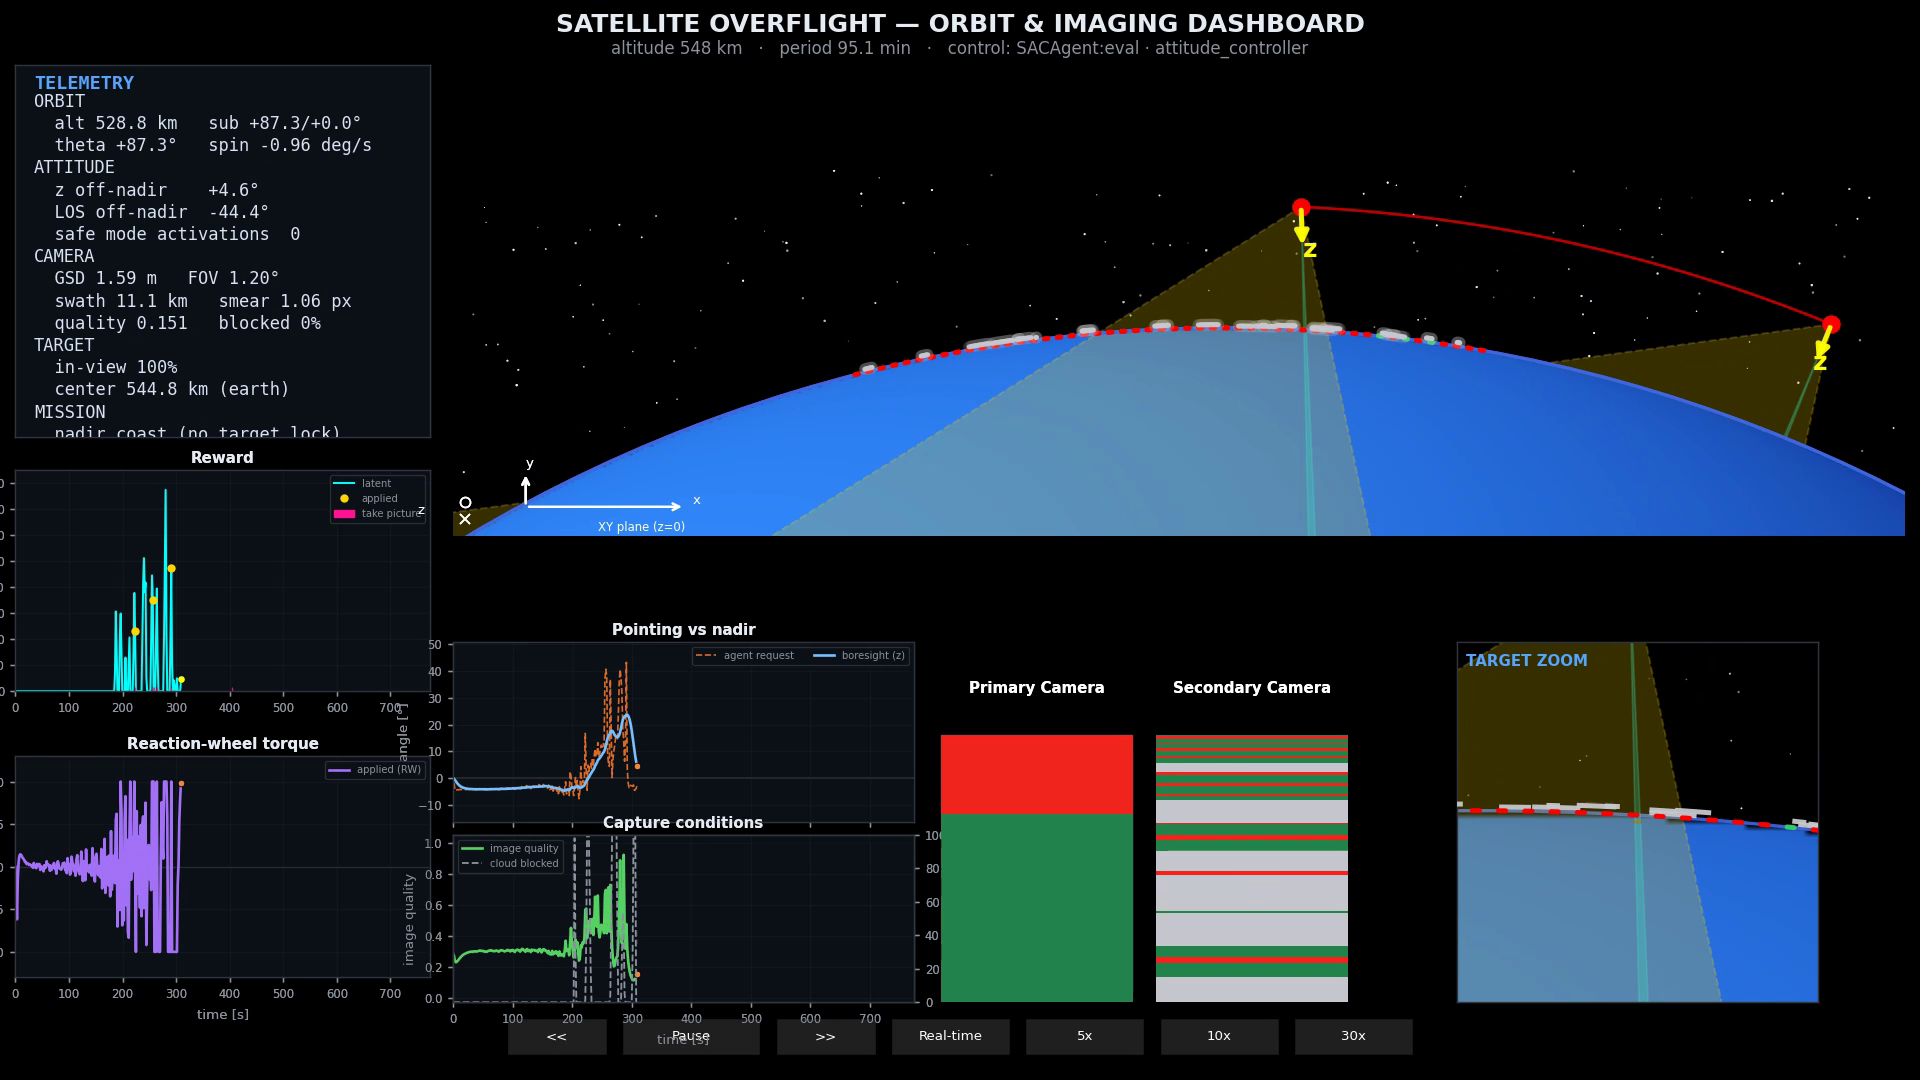
\includegraphics[width=0.88\linewidth]{figures/fig_selective_shutter.png}
  \caption{Eval episode from Exp~9 (SAC shutter-split): representative dashboard frame during selective capture behaviour on the fixed evaluation seed.}
  \label{fig:selective-shutter}
\end{figure}

\subsection{Safe-mode and safety overhead}
\label{sec:results-safemode}

In torque mode (Exps~1--5, 8) the safety controller activates 5--6 times per episode,
locking out the agent for 60\,s per event (Section~\ref{sec:safety}).
Each lockout consumes $\approx$40 controller steps with no capture opportunity.
With 516 steps per episode and 5 lockouts, approximately 40\% of the episode is unavailable to the agent.

Vector mode (Exps~4 Ref1, 7, 9, 11, 12) eliminates safe-mode lockouts in the experiment runs:
the hold-last semantics prevent the pointing reference from exceeding $\theta_\text{hard}$,
so the safety controller is never triggered.

This structural difference explains much of the torque-versus-vector gap.
The safe-mode penalty (Exp~10) attempted to replicate this improvement via reward shaping
but produced the worst result in the series ($-510.4$), confirming that action-space redesign (vector mode) is preferable to reward penalties for aligning safety and learning.

\subsection{Algorithm comparison: SAC vs.\ MPO}
\label{sec:results-algo}

At matched protocol (sparse, vector, 50 episodes, seed~7), the best SAC configuration (Exp~9, $+106.4$) exceeds the best MPO configuration (Exp~11, $+45.5$) on eval return by 60.9 points.
The gap is partially explained by reward configuration: Exp~9 uses the waste-off, budget-on reward while Exp~11 uses the budget-on, waste-on default.
An MPO run with the Exp~9 reward settings was not completed within the project timeline.

Both best configurations exceed the baseline anchor on this seed ($-38.6$).
That is encouraging for the design search but not sufficient evidence of robust mission-level superiority: evaluation uses only two episodes at a fixed seed, and several intermediate configurations never learned at all.
The more durable finding is behavioural.
Both algorithms can learn selective shuttering once reward and action-space choices are correct.
That is a stronger claim than reliable baseline outperformance under all training conditions.
